% Number 840
% CAPMA Algebra Units 
% Model rocket - thrust plus freefall, algebraic
% JG

% Watermark
\AddToShipoutPicture*{\BackgroundPic}

\addtocounter {ProbNum} {1}

%\begin{floatingfigure}[r]{.44\textwidth}
%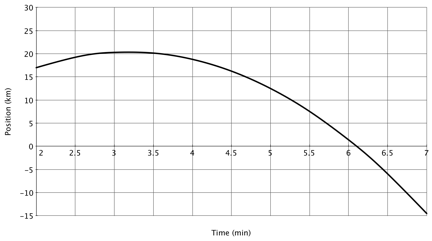
\includegraphics[scale=.5]{/Users/jgates/desktop/latex/pics/xgraph2}
%\end{floatingfigure}
 
{\bf \Large{\arabic{ProbNum}}} A model rocket lifts off and flies with an acceleration of ${12~\tfrac{m}{s^2}}$, until it reaches a height of 26 meters, at which time it continues its flight without any engine thrust.    \bigskip

What maximum speed does the rocket reach?\paragraph{}
\noindent
\vfill

What maximum height does it reach?

\vfill
%\begin{center}
%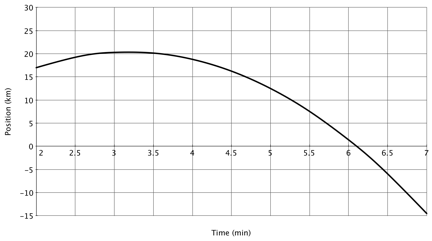
\includegraphics[scale=1]{/Users/jgates/desktop/latex/pics/xgraph2}
%\end{center}


\newpage